\documentclass[tikz,border=4pt]{standalone}
\usetikzlibrary{positioning}

\begin{document}
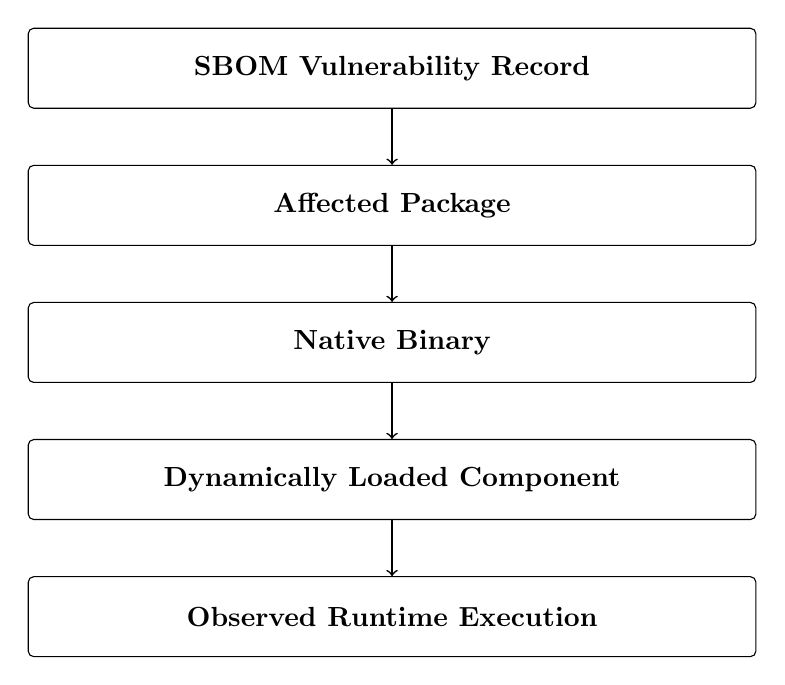
\begin{tikzpicture}[
  stage/.style={
    draw,
    rounded corners=2pt,
    text width=3.5in,
    minimum height=0.4in,
    align=center,
    font=\bfseries,
    inner sep=5pt
  },
  node distance=0.28in
]
\node[stage] (sbom) {SBOM Vulnerability Record};
\node[stage, below=of sbom] (package) {Affected Package};
\node[stage, below=of package] (binary) {Native Binary};
\node[stage, below=of binary] (component) {Dynamically Loaded Component};
\node[stage, below=of component] (runtime) {Observed Runtime Execution};

\draw[->, semithick] (sbom) -- (package);
\draw[->, semithick] (package) -- (binary);
\draw[->, semithick] (binary) -- (component);
\draw[->, semithick] (component) -- (runtime);
\end{tikzpicture}
\end{document}
